\section{Mathematical Models}
\label{ch:mathmodel}

As per the base and periodic models shown in \cite{grigor20}.

\subsection{Base model}

\subsubsection{Model Assumptions}
\begin{itemize}
    \item[(I)] Any infected person becomes ill (symptomatic) and infectious on the $q$-th day after infection.
    \item[(A)] During each day, each ill person unconfined infects on average $a$ other persons.
    \item[(B)] During each day, a proportion $b\in (0,1)$ of ill people loose gets isolated (hospitalized or otherwise) and withdrawn from a further spread of the epidemic.
\end{itemize}

\begin{nremark}
The number of days before an infected person becomes infectious is called the \textit{latent period}, and before he/she becomes symptomatically ill – the \textit{incubation period}. Here we assume for simplicity that these two periods are equal to $q$.
\end{nremark}

Many models use a set of differential equations for to describe the movement of people between \textit{groups} or \textit{compartments}. The SIR (Susceptible–Infectious–Recovered) model, the most frequently used model in epidemiology, uses a set of 3 such differential equations. 

Our main mathematical models (and even some of the statistical models) make use of \textit{recurrence equations}, which have some correspondence to differential equations \cite{AGARWAL20021}.

\subsubsection{Notation}
\begin{itemize}
    \item $x_n$ - the number of infected people that are detected and isolated during the day $n$;
    \item $y_n$ – the cumulative number of detected cases from the beginning of epidemic by the beginning of the day $n$;
    \item $z_n$ – the number of ill people at large by the beginning of the day $n$ (that is, those who were infected at least $q$ days ago and stay unisolated);
    \item $u_n$ – the number of people newly infected during the day $n$.
\end{itemize}

We will obtain the following relation between the leading root $r$ and the basic reproductive rate $R_0$ that is a main characteristic of an epidemic in epidemiology:

\begin{equation}\label{eq:R0}
    r \approx R_0^{\frac1{2q}}.
\end{equation}

Recurrence relation for $z_n$:

The number of ill people at large on day $n+1$ is the number at large on day $n$, minus the number who were detected and isolated on day $n$, plus the number of people who were infected $q$ days ago, i.e. 

\begin{equation} \label{eq:znrecurr}
    z_{n+1} = z_n - x_n + u_{n-q}.
\end{equation}

Using $x_n = bz_n$ and $u_{n-q} = ax_{n-q}$ we obtain the following equation for $x_n$:
\begin{equation} \label{eq:xnrecurr}
    x_{n+1} = (1 - b) x_n + ax_{n-q}.
\end{equation}

It is necessary to let the model equal the actual data for the first $q+1$ days, as the recurrence equation needs initial data:
\begin{equation} \label{eq:xn0q}
x_n = x^*_n \ \text{for} \ n = 0, 1, \dots , q,
\end{equation}

 To fit our model we optimize against the average 1-norm:
\begin{equation}\label{eq:xnnorm}
    \norm{x-x^*}:= \frac{1}{N+1} \sum\limits_{n=0}^N |x_n-x_n^*|, \quad N\in \mathbb{N},
\end{equation}

Similarly we define $\norm{y-y^*}$

We choose $N$ to be the length of the data (number of actual observations $x_n^*$) in general.

In order to determine values $a,b,q$, we ideally want to minimize both 

\begin{equation} \label{eq:norms}
    \norm{x-x^*} \ \text{and} \ \norm{y-y^*}
\end{equation}

While this is the ideal situation, it is far more important to minimize $\norm{x-x^*}$ as it is generally much more sensitive to variation in the parameters (such as $a$ and $b$).


The proofs and results are in \ref{ch:theorems}.

\subsubsection{How to select the best model}

The closest-fiting model will be one that minimizes \eqref{eq:xnnorm}, which can bee seen using contour plots below.

\begin{figure}[H]
\minipage{0.33\textwidth}
  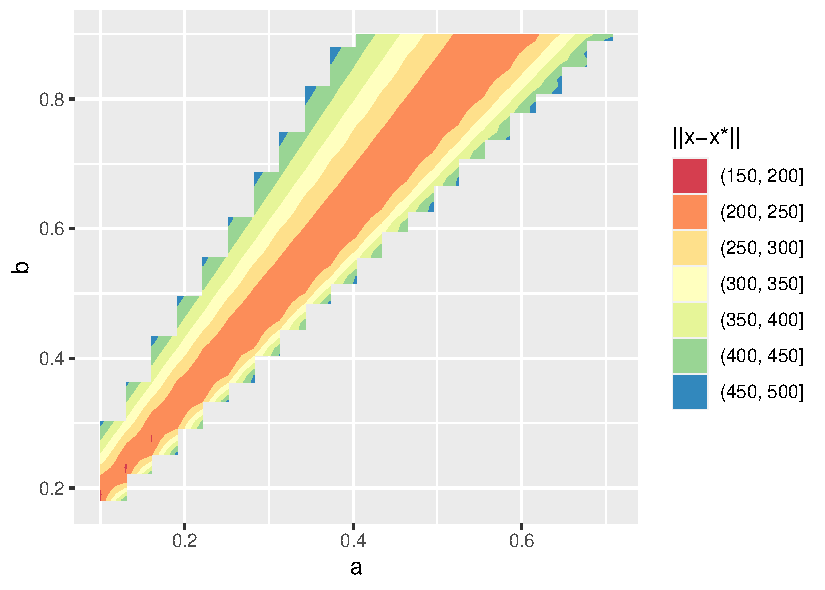
\includegraphics[width=\linewidth]{Ireland-combnorm.pdf} \label{fig:ireland-combnorm}
\caption{Contours, Ireland}
\endminipage\hfill
\minipage{0.33\textwidth}
  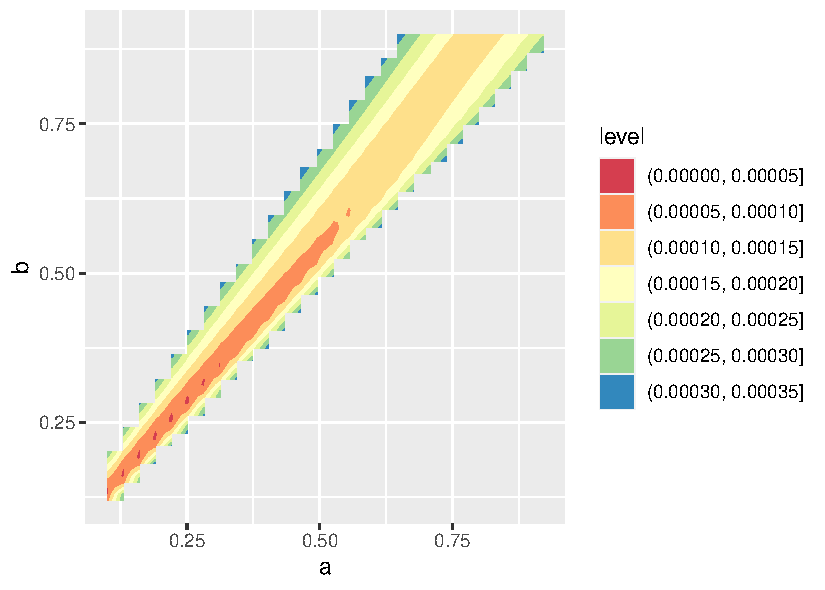
\includegraphics[width=\linewidth]{Italy-combnorm.pdf} \label{fig:italy-combnorm}
\caption{Contours, Italy}
\endminipage\hfill
\minipage{0.33\textwidth}
  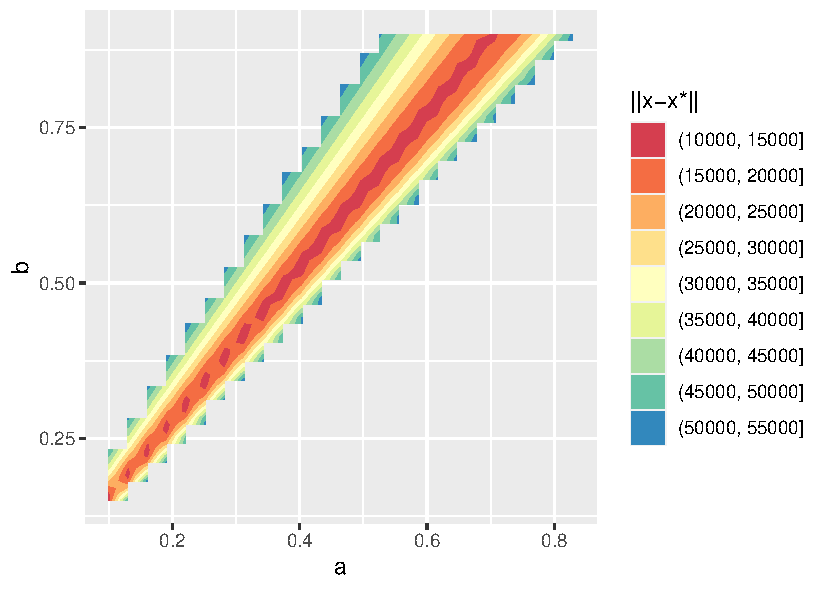
\includegraphics[width=\linewidth]{United States-combnorm.pdf} \label{fig:usa-combnorm}
\caption{Contours, United States}
\endminipage\hfill
\end{figure}

The \verb|optim()| function in \verb|R| appeared to have a danger of converging to local optima, so with some trade-off in computation time over accuracy, I have chosen to iterate the algorithm \verb|basicmodx()| over all combinations of $a,b,q$.

\subsubsection{Forecasting}

The model can easily be extended $m$ days ahead, with $x_{N+1},\dots,x_{N+m}$ defined recursively using \ref{eq:xnrecurr}.

\subsubsection{Implementation in R}

\begin{lstlisting}[breaklines = true, escapeinside=||, tabsize = 4, caption = {Algorithm for Base Model}]
basicmodx <- function(x, pars, len = 0){
  q <- floor(pars[1])
  a <- pars[2]
  b <- pars[3]
  modx <- x[1:q]
  for(i in (q+1):(length(x)+len)){
    modx[i] <- (1-b)*modx[i-1] + a*modx[i-q]
  }
  return(modx)
}
basexn   <- basicmodx(countrydat$xn, optimpars, len = forecastlen)  |\Suppressnumber|
...
...
...|\Reactivatenumber|
plots[["basexn"]] <- plot_basexn(countrydat, modeldat, cols, labs)
\end{lstlisting}

\subsubsection{Plots}

\begin{figure}[H]
\minipage{0.48\textwidth}
  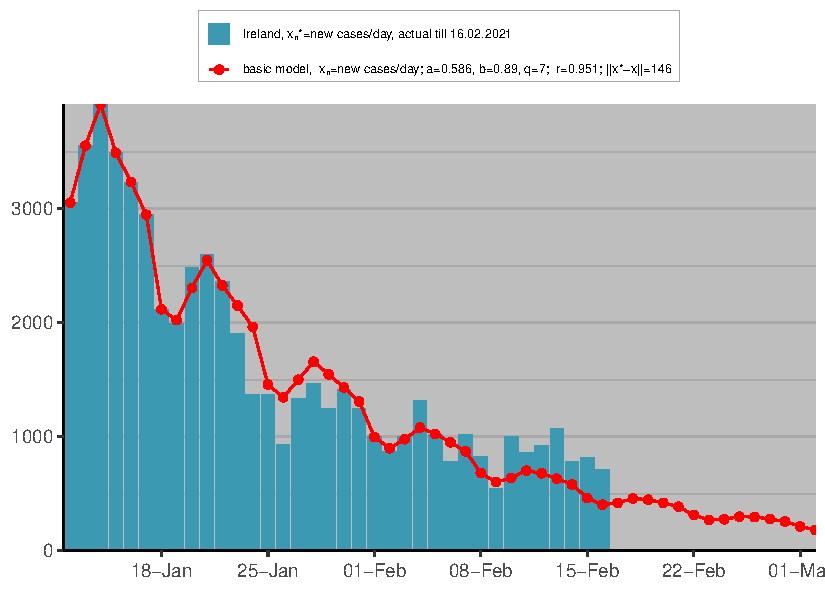
\includegraphics[width=\linewidth]{Ireland-basexn.pdf} \label{fig:ireland-basexn}
\endminipage\hfill
\minipage{0.48\textwidth}
  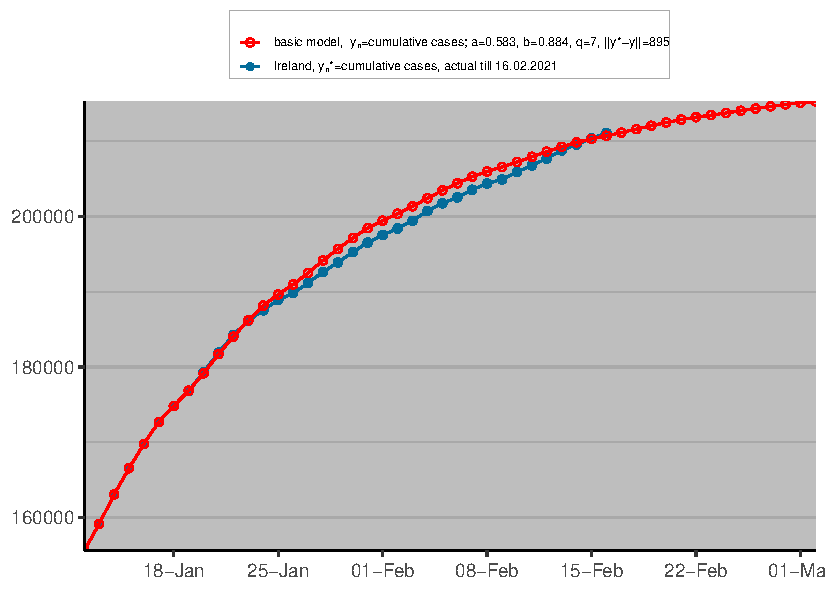
\includegraphics[width=\linewidth]{Ireland-baseyn.pdf} \label{fig:ireland-baseyn}
\endminipage
\caption{Basic model, Ireland}
\end{figure}

\begin{figure}[H]
\minipage{0.48\textwidth}
  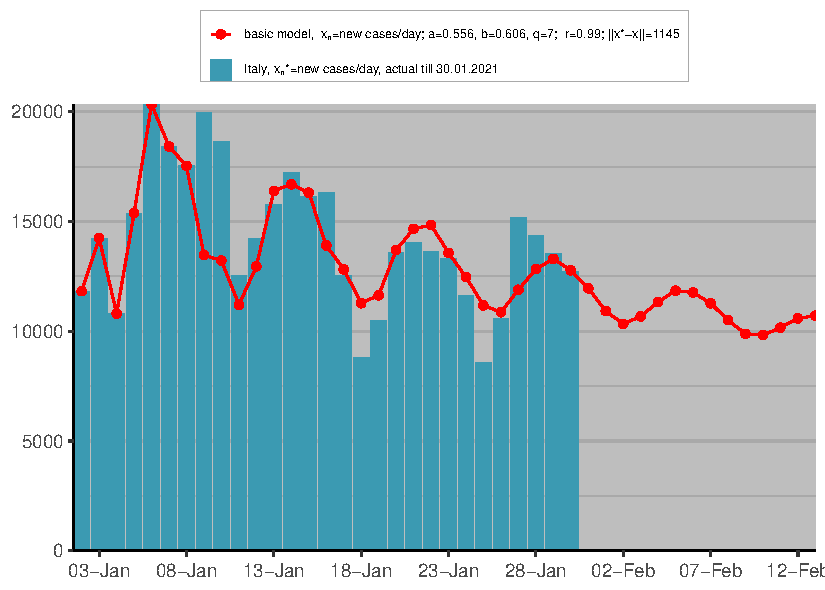
\includegraphics[width=\linewidth]{Italy-basexn.pdf} \label{fig:italy-basexn}
\endminipage\hfill
\minipage{0.48\textwidth}
  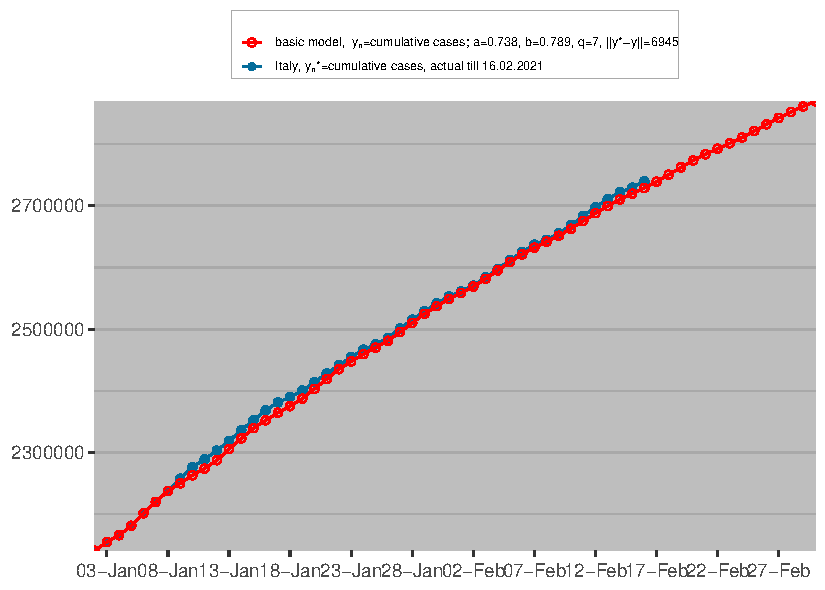
\includegraphics[width=\linewidth]{Italy-baseyn.pdf} \label{fig:italy-baseyn}
\endminipage
\caption{Basic model, Italy}
\end{figure}

\begin{figure}[H]
\minipage{0.48\textwidth}
  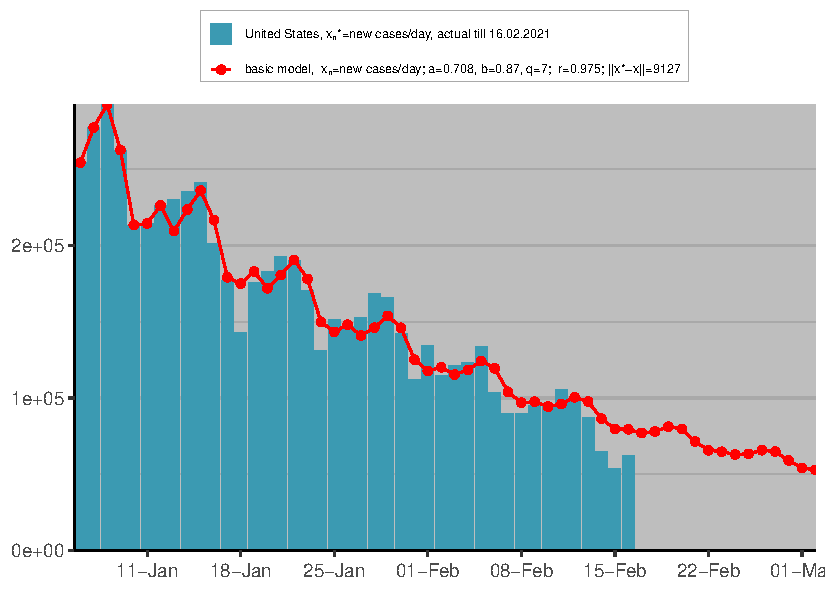
\includegraphics[width=\linewidth]{United States-basexn.pdf} \label{fig:usa-basexn}
\endminipage\hfill
\minipage{0.48\textwidth}
  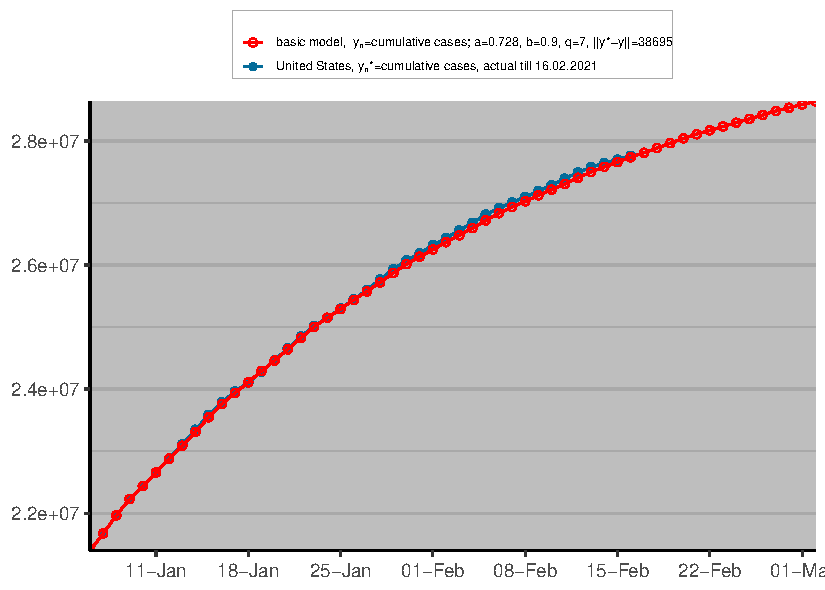
\includegraphics[width=\linewidth]{United States-baseyn.pdf} \label{fig:usa-baseyn}
\endminipage
\caption{Basic model, United States}
\end{figure}

\subsection{Limiting curve \ce{Cr^n}}

The second result in \ref{thm:lim} is the equation \eqref{eq:crn}, which defines the limiting behavior of the recurrence relation \eqref{eq:xnrecurr}.

\begin{lstlisting}[breaklines = true, escapeinside=||, tabsize = 4, caption = {Algorithm for Limiting Curve}]
modeldat$Crn <- optimC*base_r_one^(1:nrow(modeldat))  |\Suppressnumber|
...
...
...|\Reactivatenumber|
plots[["Crn"]] <- plot_crn(countrydat, modeldat, cols, labs)
\end{lstlisting}

\begin{figure}[H]
\minipage{0.33\textwidth}
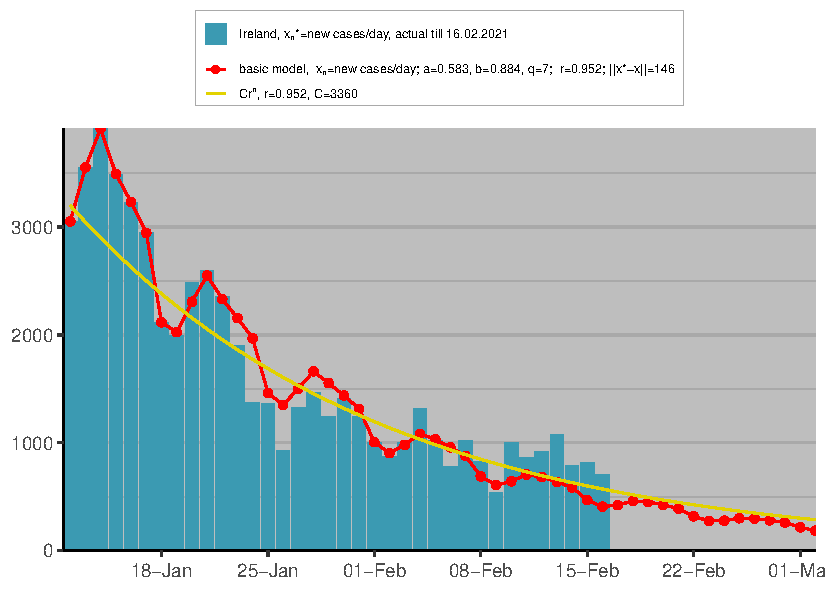
\includegraphics[width=0.9\textwidth]{Ireland-Crn.pdf}
\caption{Limiting curve $Cr^n$, Ireland}
\endminipage 
\minipage{0.33\textwidth}
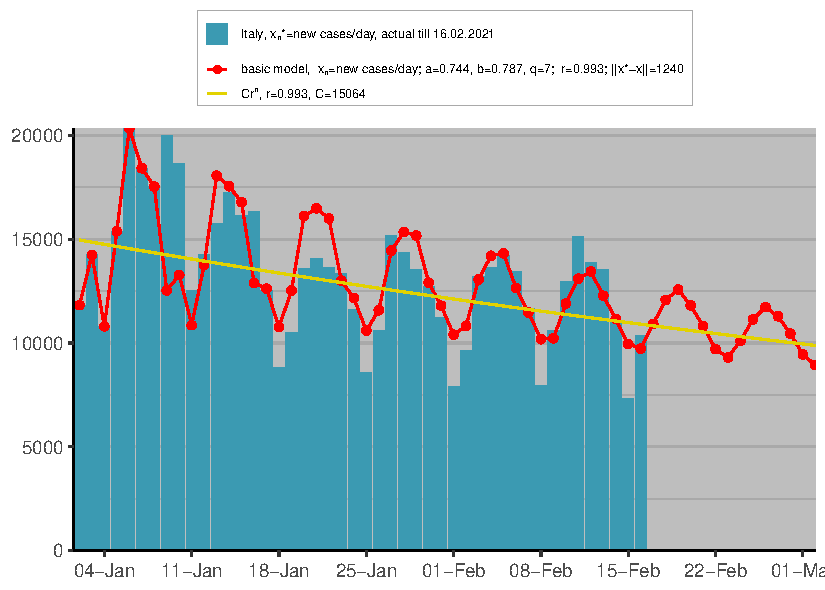
\includegraphics[width=0.9\textwidth]{Italy-Crn.pdf}
\caption{Limiting curve $Cr^n$, Italy}
\endminipage 
\minipage{0.33\textwidth}
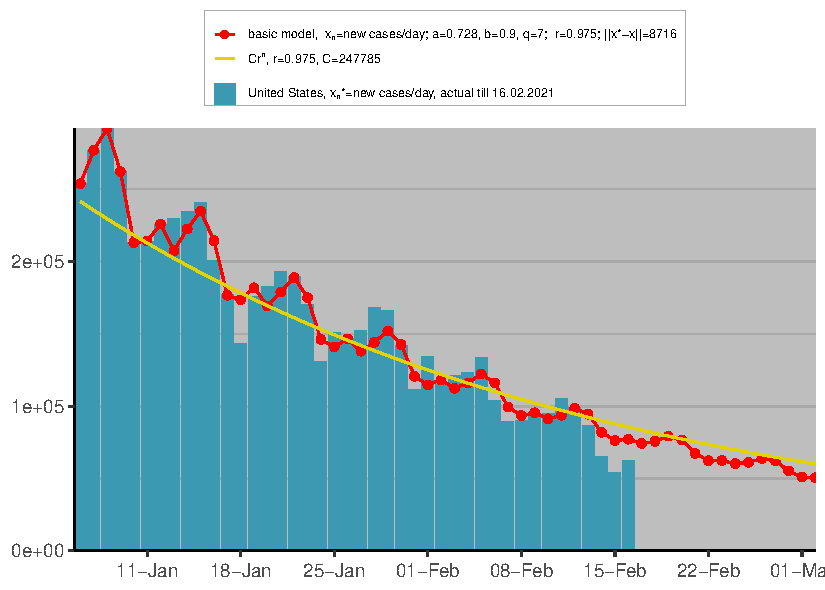
\includegraphics[width=0.9\textwidth]{United States-Crn.pdf}
\caption{Limiting curve $Cr^n$, United States}
\endminipage 
\end{figure}

The limiting curve can also show exponential growth and quickly get out of control

\begin{figure}[H]
\minipage{0.98\textwidth}
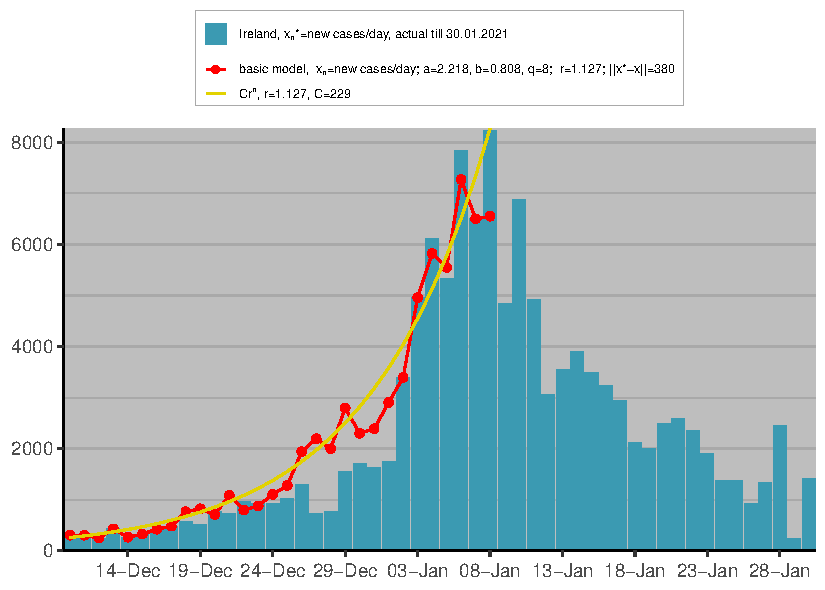
\includegraphics[width=0.9\textwidth]{Ireland-expgrowth.pdf}
\endminipage 
\caption{Limiting Curve Growing Exponentially, Ireland}
\end{figure}

\subsection{Moving average}

Define the $2k+1$-day moving average of actual data $x_n^*$ by $x^*(k)$

$\begin{aligned}
x^*_n(1) &=\frac{x^*_{n-1} + x^*_n + x^*_{n+1}}{3},\quad 1\leq n < N \\
x^*_0(1) &=\frac{x^*_0 + x^*_1}{2}\\
x^*_N(1) &=\frac{x^*_{N-1} + x^*_N}{2}
\end{aligned}$

And then $$x_n^*(3):= x^*_n(x^*_n(1))$$ is the 7-day moving average of cases.

The 7-day moving average is a good baseline for model performance , as ideally we would want $\norm{x-x^*}\approx\norm{x^*(3)-x^*}$ or better.

\begin{figure}[H]
\minipage{0.33\textwidth}
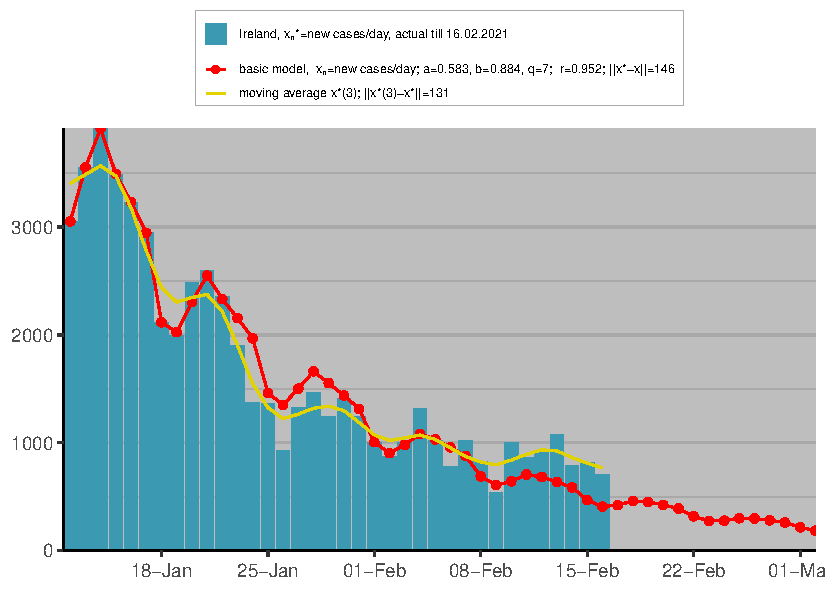
\includegraphics[width=0.9\textwidth]{Ireland-mavgx3.pdf}
\caption{Moving average $x^*_n(3)$, Ireland}
\endminipage 
\minipage{0.33\textwidth}
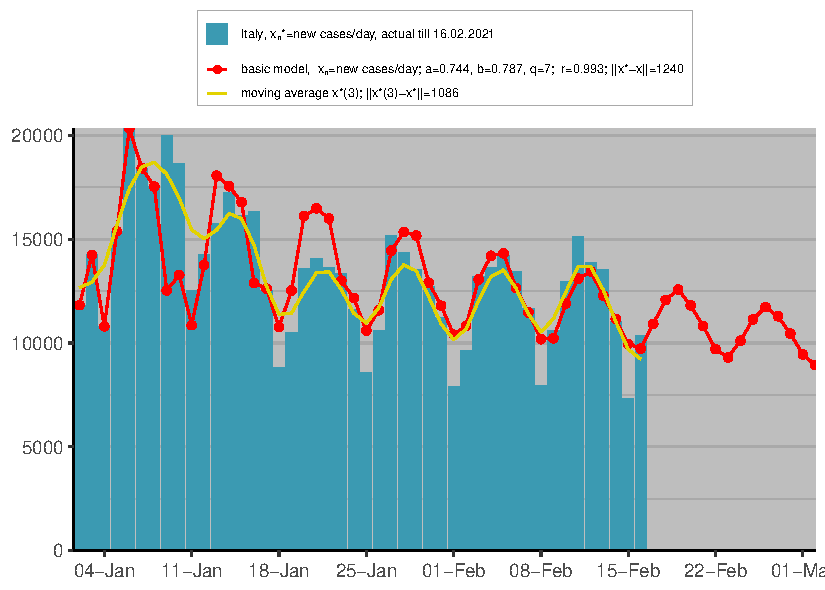
\includegraphics[width=0.9\textwidth]{Italy-mavgx3.pdf}
\caption{Moving average $x^*_n(3)$, Italy}
\endminipage 
\minipage{0.33\textwidth}
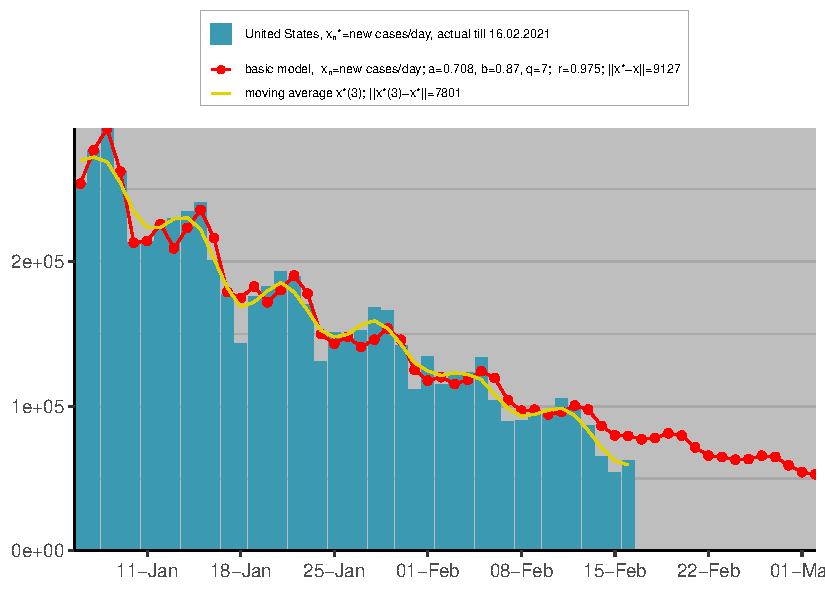
\includegraphics[width=0.9\textwidth]{United States-mavgx3.pdf}
\caption{Moving average $x^*_n(3)$, United States}
\endminipage 
\end{figure}

\subsection{Periodic model}\label{ch:periodic}

Instead of constant parameters $a,b$, we vary them slightly over time:

\begin{equation} \label{eq:anper}
a_n := a\rbr{1+c_1\rbr{\sin\rbr{\frac{2\pi}{p_1}\rbr{n-n_1}}}}
\end{equation}

\begin{equation} \label{eq:bnper}
b_n := b\rbr{1+c_2\rbr{\sin\rbr{\frac{2\pi}{p_2}\rbr{n-n_2}}}}
\end{equation}

\begin{figure}[H]
\minipage{0.33\textwidth}
  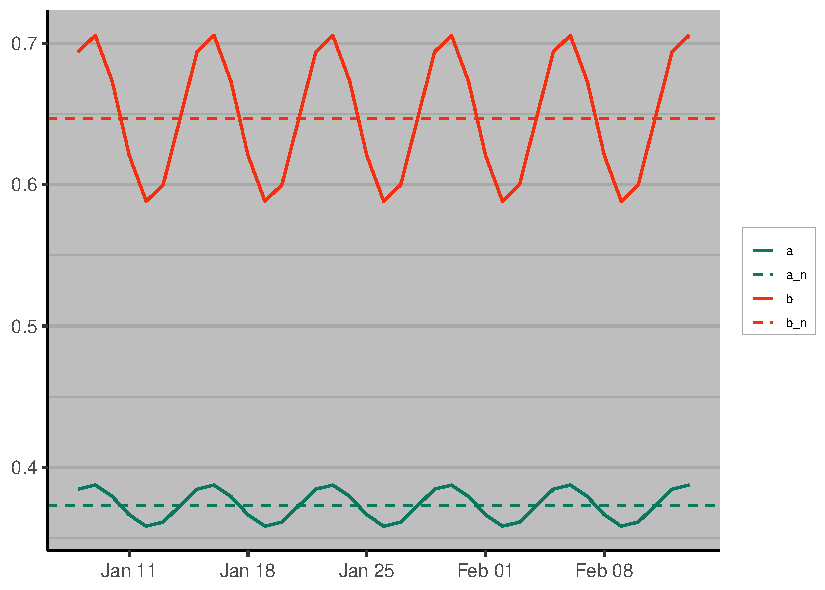
\includegraphics[width=\linewidth]{Ireland-perparam.pdf} \label{fig:ireland-perparam}
\endminipage\hfill
\minipage{0.33\textwidth}
  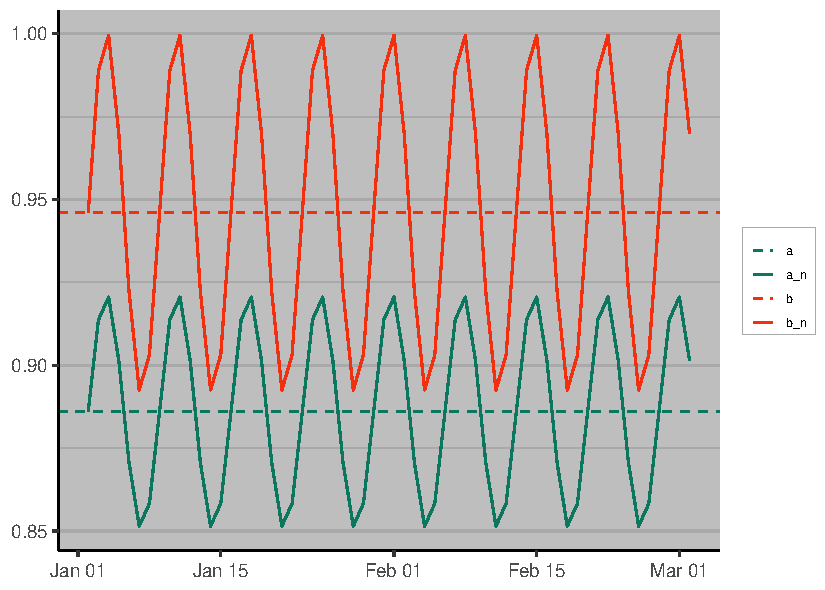
\includegraphics[width=\linewidth]{Italy-perparam.pdf} \label{fig:italy-perparam}
\endminipage\hfill
\minipage{0.33\textwidth}
  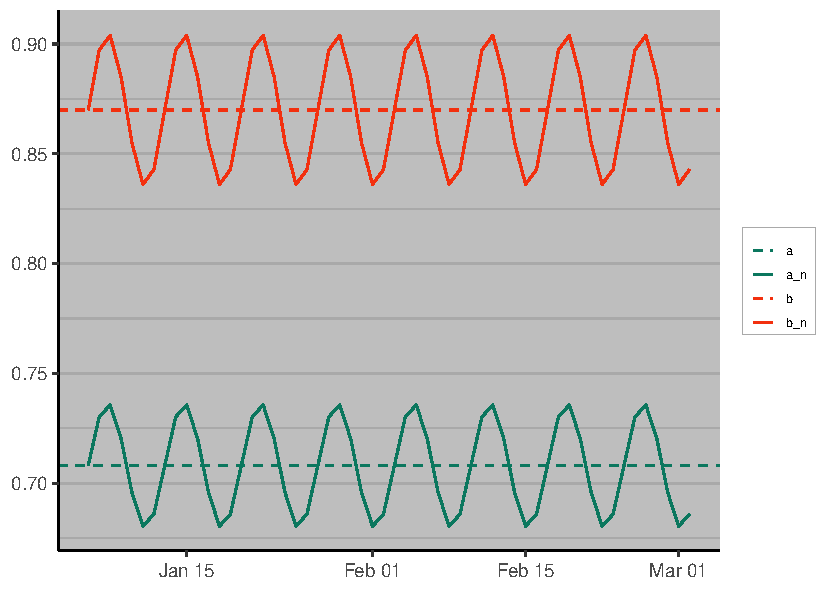
\includegraphics[width=\linewidth]{United States-perparam.pdf} \label{fig:usa-perparam}
\endminipage\hfill
\caption{Oscillating $a$ and $b$ parameters, Ireland, Italy and United States}
\end{figure}

For new parameters $c_i,p_i,n_i, \ i=1,2$ where

$c_i  \in [0.04, 0.2]$ \quad are (small) amplitudes,

$n_i  \in 1,2,\dots,q$ \quad  are lags and

$p_i  \in 1,2,\dots,q$ \quad are periods.

We then have to optimize \eqref{eq:norms} with respect to the $9$ parameters $a,b,q,c_1,n_1,p_1,c_2,n_2$ and $p_2$.

While Grigorian's paper \cite{grigor20} optimized with (possibly) new values of $a$ and $b$, I will allow the original $a$ and $b$ from the earlier optimization to calculate the $a_n$ and $b_n$,since the average behavior should be close to the same. 

I included a sketch of the proof in the appendix \ref{thm:avgparam}.

This means that we can keep the original parameters $a,b,q$ (we assume the latency period is constant), and we are instead optimizing over the $6$ parameters $c_1,n_1,p_1,c_2,n_2,p_2$

This enables the algorithm to speed up by at least an order of magnitude.

\subsubsection{Implementation in R}

\begin{lstlisting}[breaklines = true, escapeinside=||, tabsize = 4, frame=single, caption = {Algorithm for Periodic Model}]
modxper <- function(par, q, x, len = 0){
  #a,b,c1,c2,p1,p2,n1,n2
  an   <- par[1]*(1+par[3]*sin(2*pi*(1:(length(x)+len) - par[7])/par[5]))
  bn   <- par[2]*(1+par[4]*sin(2*pi*(1:(length(x)+len) - par[8])/par[6]))
  modx <- x[1:q]
  for(i in (q+1):(length(x)+len)){
    modx[i] <- (bn[i]*(1-bn[i-1]))*modx[i-1]/bn[i-1] +
      (an[i-q]*bn[i])*modx[i-q]/bn[i-q]
  }
  return(modx)
}
modeldat$periodic  <- modxper(as.numeric(peroptim),countrydat$xn, q = q, forecastlen)|\Suppressnumber|
...
...
...|\Reactivatenumber|
plots[["periodic"]] <- plot_periodic(countrydat, modeldat, cols, labs)
\end{lstlisting}

\subsubsection{Plots}

\begin{figure}[H]
\minipage{0.48\textwidth}
  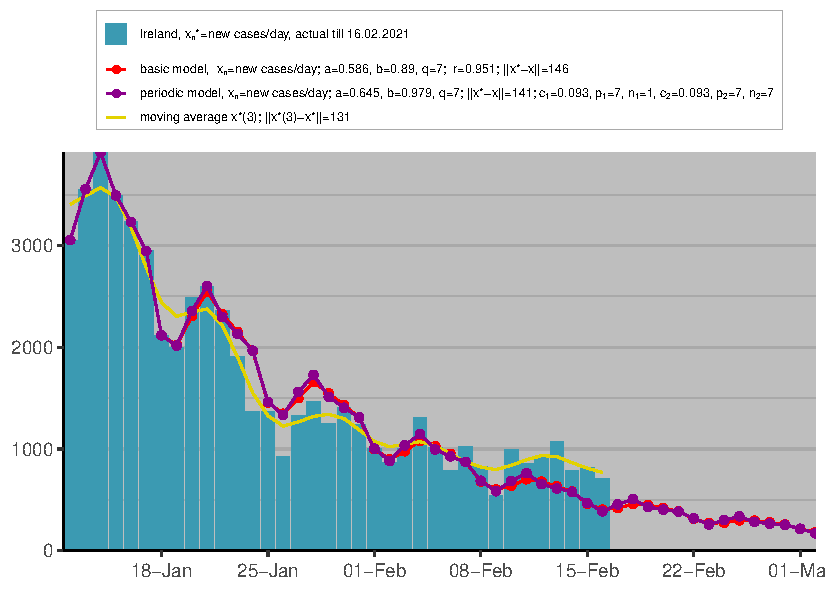
\includegraphics[width=\linewidth]{Ireland-periodic.pdf} \label{fig:ireland-periodic}
\endminipage\hfill
\minipage{0.48\textwidth}
  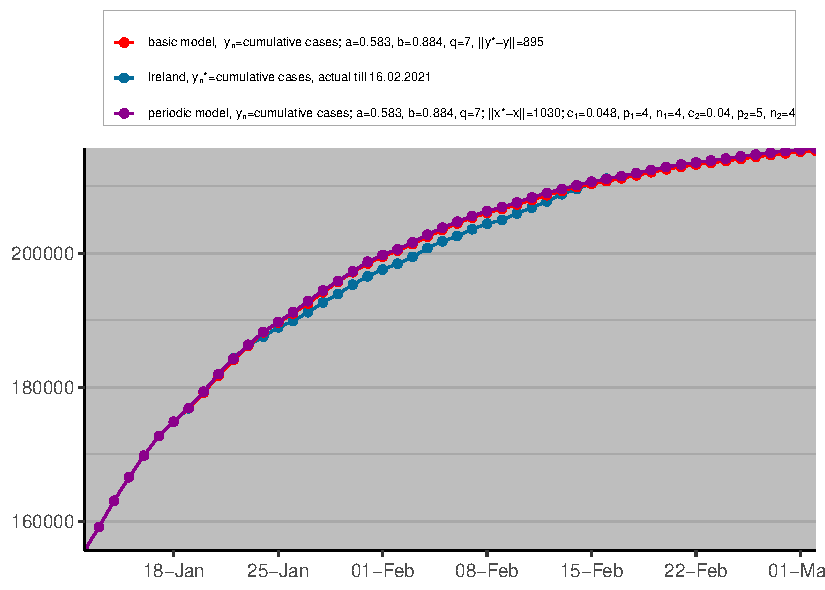
\includegraphics[width=\linewidth]{Ireland-periodicy.pdf} \label{fig:ireland-periodicy}
\endminipage
\caption{Periodic model, Ireland}
\end{figure}

\begin{figure}[H]
\minipage{0.48\textwidth}
  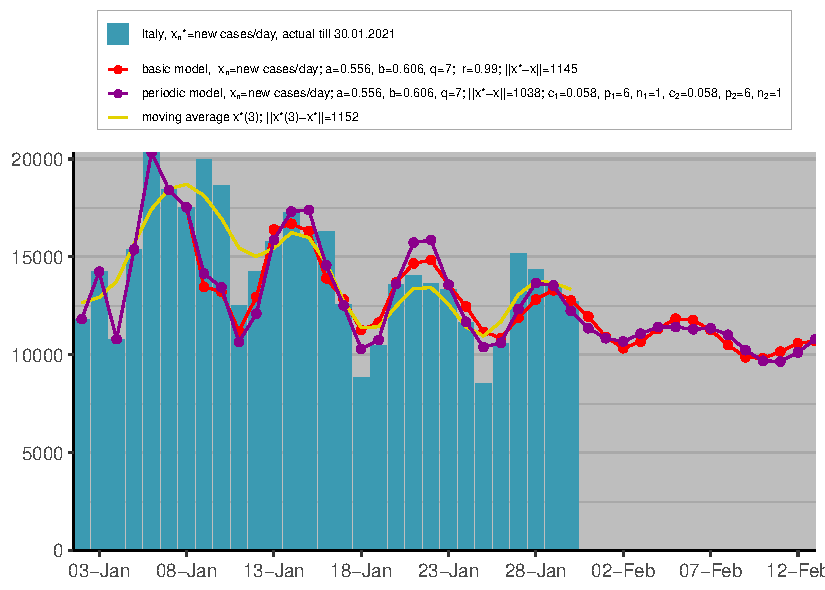
\includegraphics[width=\linewidth]{Italy-periodic.pdf} \label{fig:italy-periodic}
\endminipage\hfill
\minipage{0.48\textwidth}
  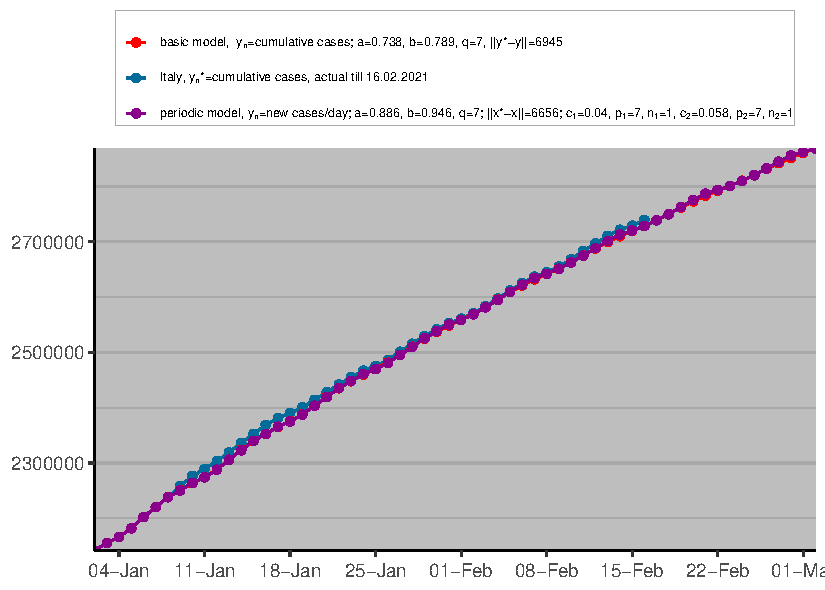
\includegraphics[width=\linewidth]{Italy-periodicy.pdf} \label{fig:italy-periodicy}
\endminipage
\caption{Periodic model, Italy}
\end{figure}

\begin{figure}[H]
\minipage{0.48\textwidth}
  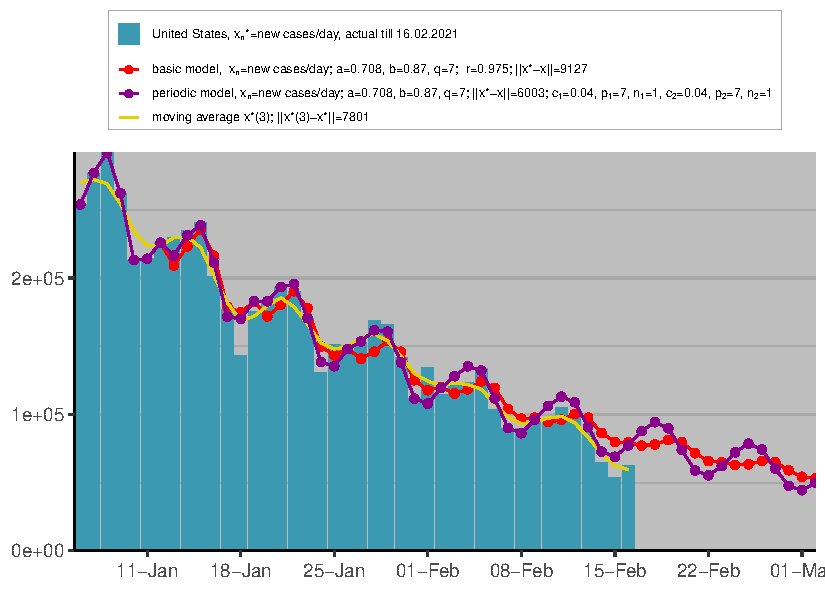
\includegraphics[width=\linewidth]{United States-periodic.pdf} \label{fig:usa-periodic}
\endminipage\hfill
\minipage{0.48\textwidth}
  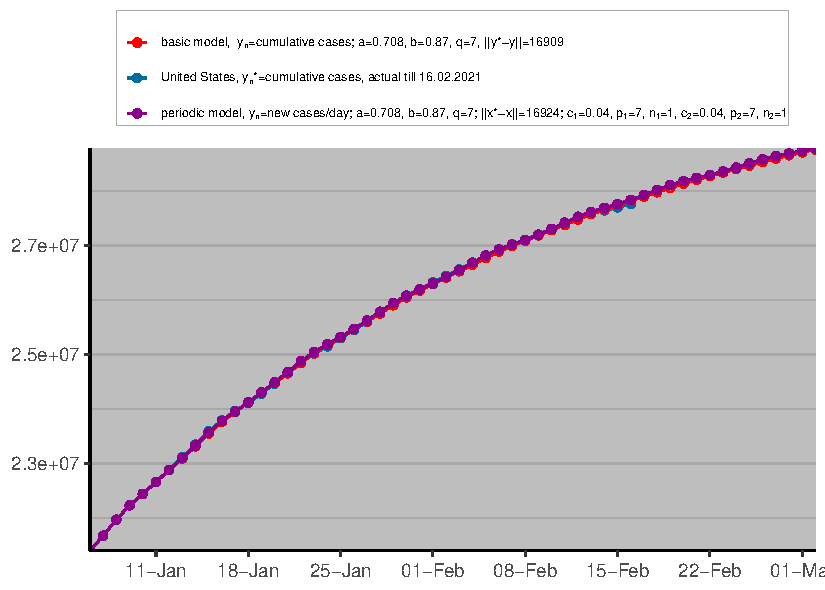
\includegraphics[width=\linewidth]{United States-periodicy.pdf} \label{fig:usa-periodicy}
\endminipage
\caption{Periodic model, United States}
\end{figure}

\subsection{Multi-phase model}

I have generalized the two-phase model formulated in \cite{grigor20} to any number of phases, both in the equations below and the code.

Suppose there are $M$ phases of the pandemic, and we wish to compute the parameters $a,b,q$ seperately for each phase.

Therefore we have phases

\begin{itemize}
\item[(1)] parameters $a_1,b_1,q_1$ and mdel $x_n$ for $0\leq n \leq N_1$
\item[(2)]  parameters $a_2,b_2,q_2$ and mdel $x_n$ for $N_1+1\leq n \leq N_2$

$\vdots$

\item[(M)] parameters $a_M,b_M,q_M$ and mdel $x_n$ for $N_{M-1}+1\leq n \leq N_M = N$
\end{itemize}

Grigorian's paper uses a form of smoothing of parameter $b$, which is using $\frac{b_{\text{new}}}{b_{\text{old}}}$ for a few days around the change point to deal with the transition between phase.

This perturbation is already dealt with sufficiently in the periodic version so I have excluded this in the event that  $\frac{b_{\text{new}}}{b_{\text{old}}}$ is much larger than 1. 

The model parameters are computed seperately for each phase, with the values $x_n$ feeding into the next phase to continue the recursive definition (e.g. phase 2 needs some values from phase 1 of the model).

The model parameters are chosen to minimize \eqref{eq:xnnorm} for each phase, and the overall model performance displayed is computed for the model as a whole against the data as a whole.

\subsubsection{Plots}

The multi-phase model without periodicity can be sharp and unrealstic, and is purely for demonstration

\begin{figure}[H]
\minipage{0.48\textwidth}
  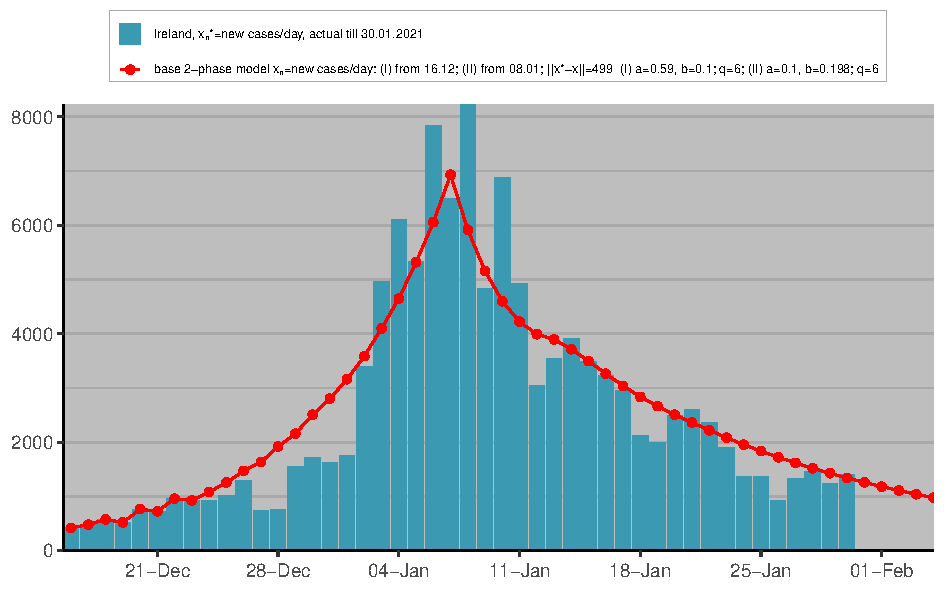
\includegraphics[width=\linewidth]{Ireland-xnmult.pdf} \label{fig:ireland-xnmult}
\endminipage\hfill
\minipage{0.48\textwidth}
  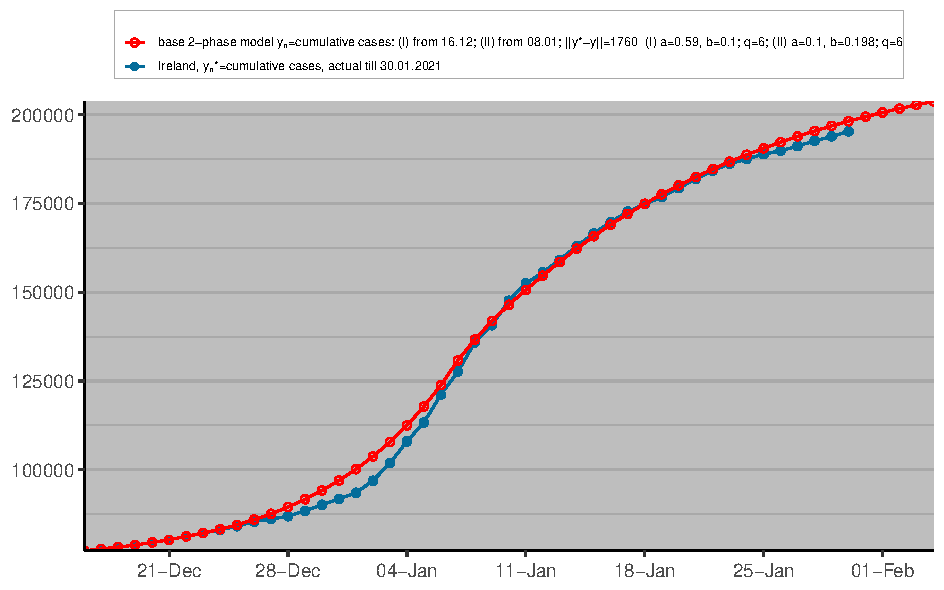
\includegraphics[width=\linewidth]{Ireland-ynmult.pdf} \label{fig:ireland-ynmult}
\endminipage
\caption{Multi-phase model, Ireland}
\end{figure}

\begin{figure}[H]
\minipage{0.48\textwidth}
  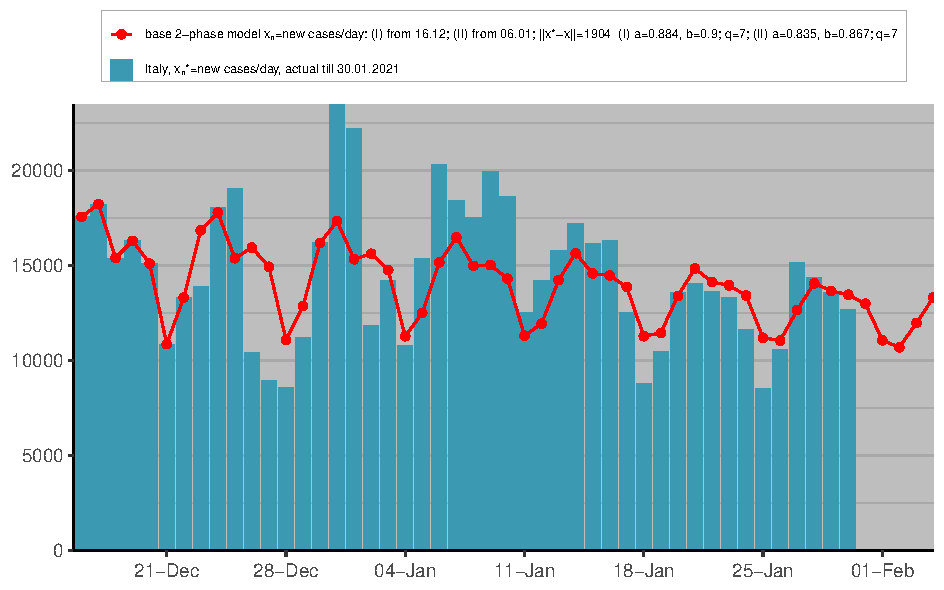
\includegraphics[width=\linewidth]{Italy-xnmult.pdf} \label{fig:italy-xnmult}
\endminipage\hfill
\minipage{0.48\textwidth}
  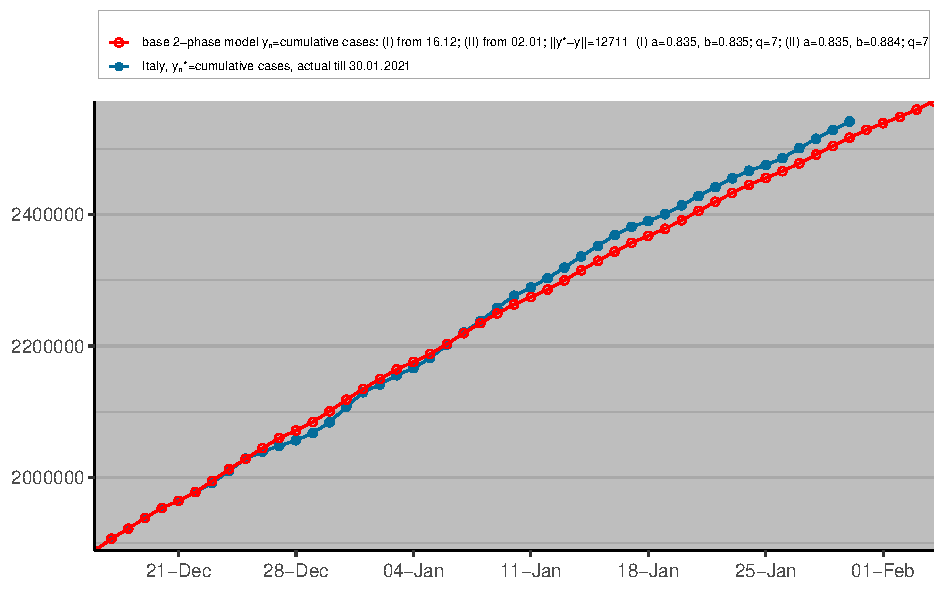
\includegraphics[width=\linewidth]{Italy-ynmult.pdf} \label{fig:italy-ynmult}
\endminipage
\caption{Multi-phase model, Italy}
\end{figure}

\begin{figure}[H]
\minipage{0.48\textwidth}
  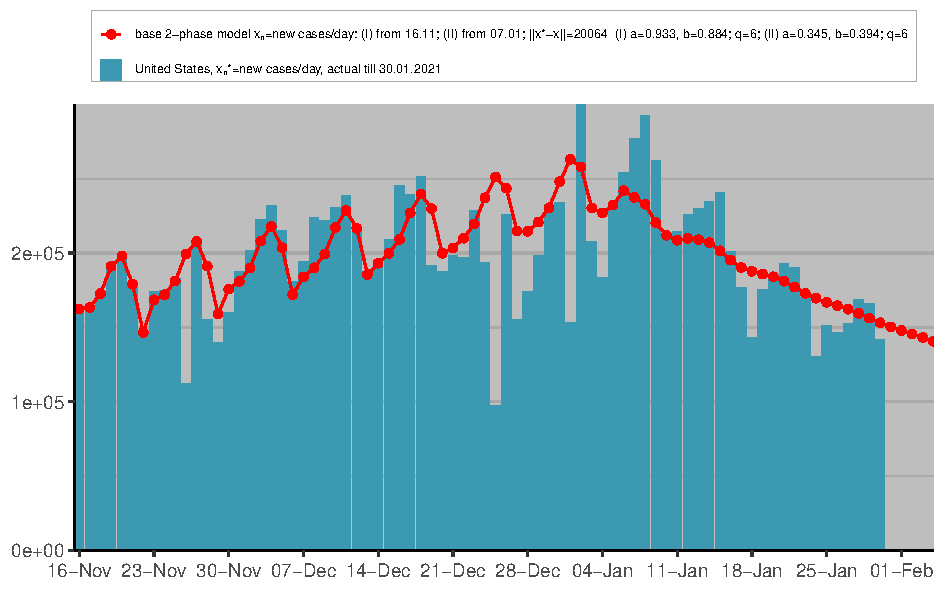
\includegraphics[width=\linewidth]{United States-xnmult.pdf} \label{fig:usa-xnmult}
\endminipage\hfill
\minipage{0.48\textwidth}
  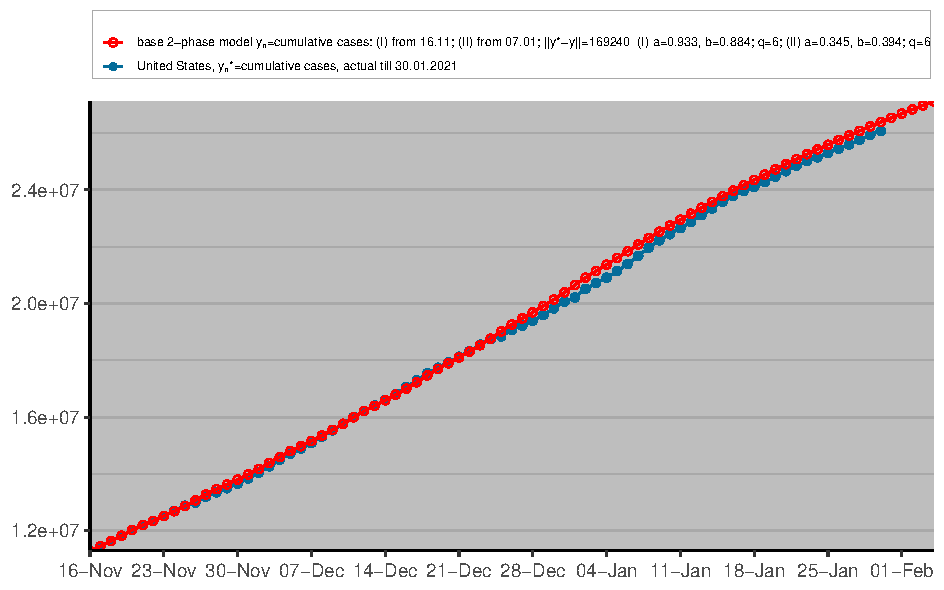
\includegraphics[width=\linewidth]{United States-ynmult.pdf} \label{fig:usa-ynmult}
\endminipage
\caption{Multi-phase model, United States}
\end{figure}

The periodic model is a similar extension as in \ref{ch:periodic} and often performs better.

\begin{figure}[H]
\minipage{0.48\textwidth}
  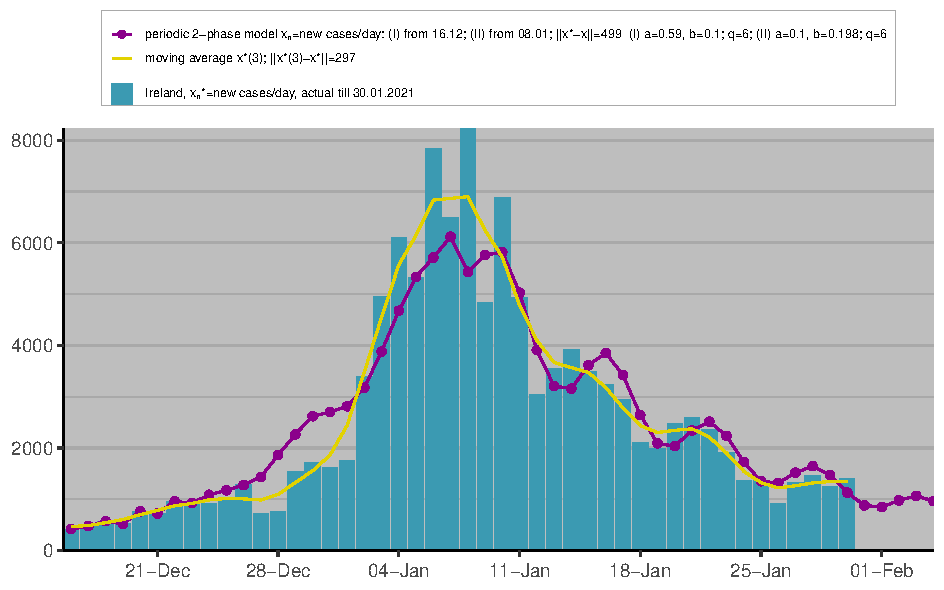
\includegraphics[width=\linewidth]{Ireland-perxnmult.pdf} \label{fig:ireland-perxnmult}
\endminipage\hfill
\minipage{0.48\textwidth}
  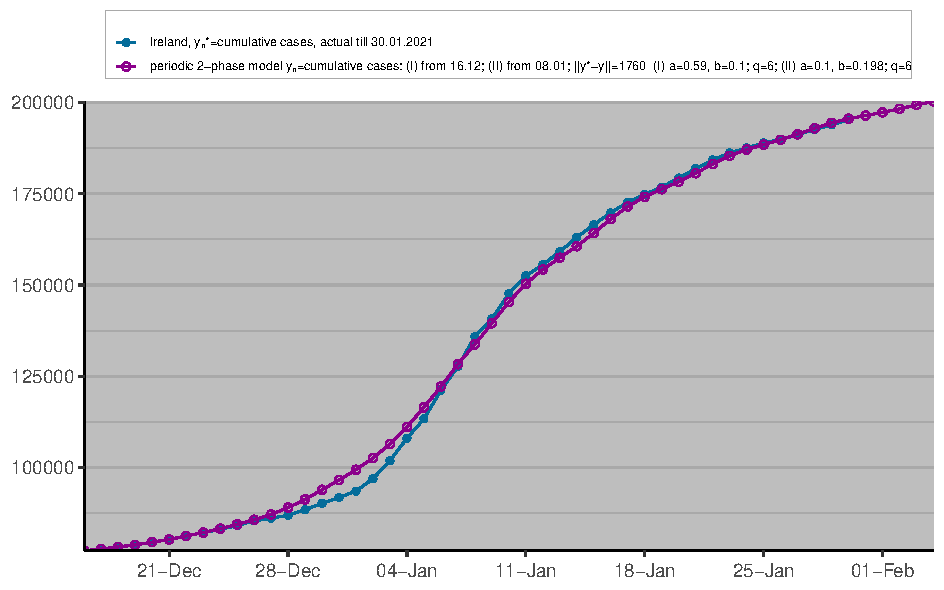
\includegraphics[width=\linewidth]{Ireland-perynmult.pdf} \label{fig:ireland-perynmult}
\endminipage
\caption{Multi-phase periodic model, Ireland}
\end{figure}

\begin{figure}[H]
\minipage{0.48\textwidth}
  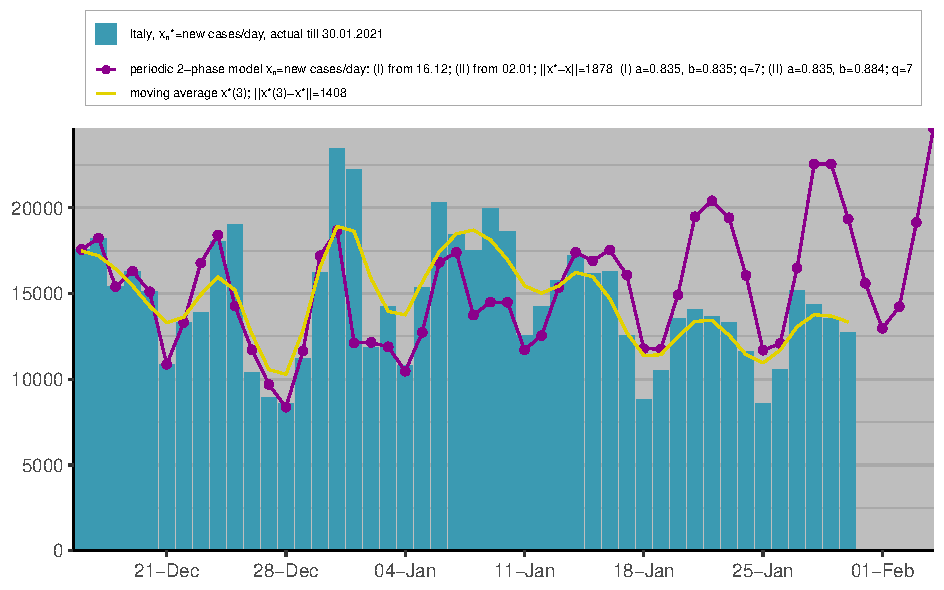
\includegraphics[width=\linewidth]{Italy-perxnmult.pdf} \label{fig:italy-perxnmult}
\endminipage\hfill
\minipage{0.48\textwidth}
  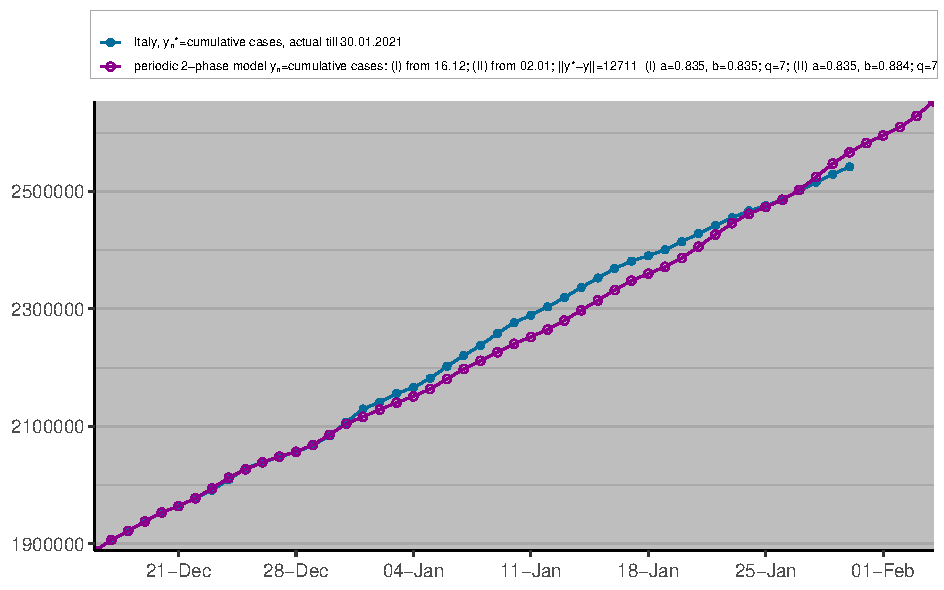
\includegraphics[width=\linewidth]{Italy-perynmult.pdf} \label{fig:italy-perynmult}
\endminipage
\caption{Multi-phase periodic model, Italy}
\end{figure}

\begin{figure}[H]
\minipage{0.48\textwidth}
  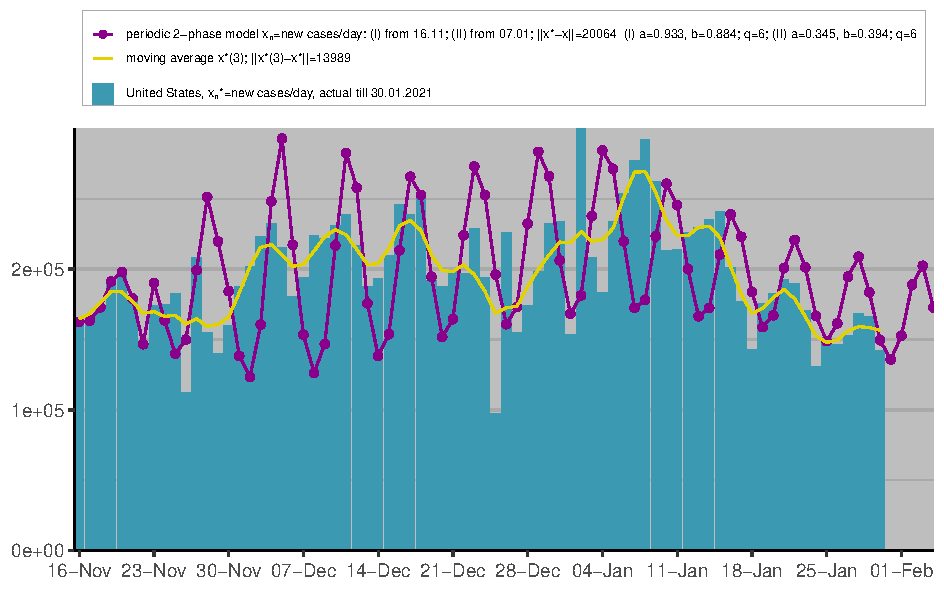
\includegraphics[width=\linewidth]{United States-perxnmult.pdf} \label{fig:usa-perxnmult}
\endminipage\hfill
\minipage{0.48\textwidth}
  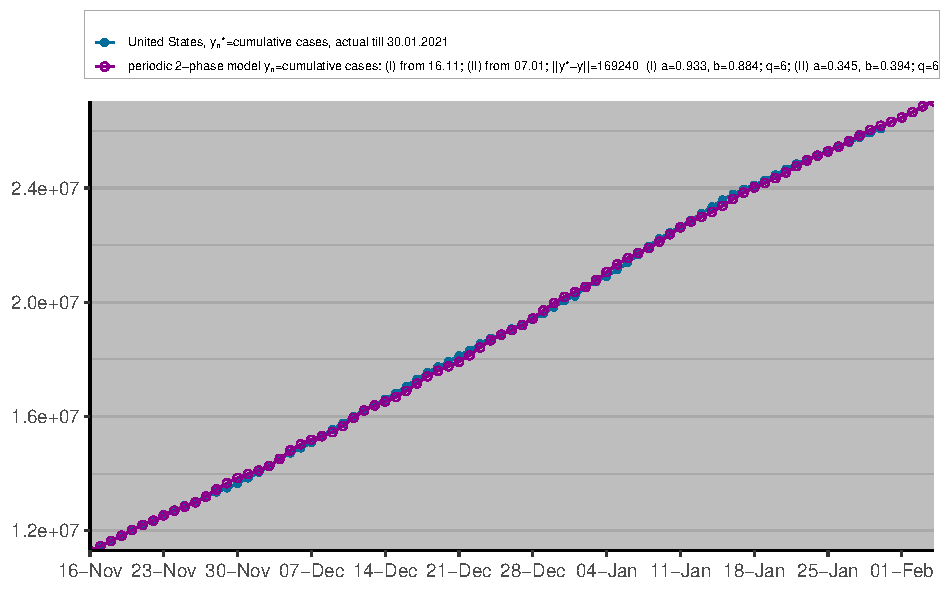
\includegraphics[width=\linewidth]{United States-perynmult.pdf} \label{fig:usa-perynmult}
\endminipage
\caption{Multi-phase periodic model, United States}
\end{figure}
